\section*{Fourier Series}
\textbf{3. Show that $B_k = \frac{2}{T_0} \oint f(t) \sin(k \omega_0 t) dt$ is consistent with the Fourier series.}
\\

\textbf{Given that:}

\begin{align}
	\int_{-T_0/2}^{T_0/2} \sin(n \omega_0 t) \sin(k \omega_0 t) dt &=
	\begin{cases}
		0,& k \neq n\\
		\frac{T_0}{2},& k = n \neq 0\\
		T_0,& k = n = 0
	\end{cases}
	\\
	\int_{-T_0/2}^{T_0/2} \cos(n \omega_0 t) \sin(k \omega_0 t) dt &= 0 
\end{align}

\begin{equation}
	\oint \equiv \int_{-T_0/2}^{T_0/2}
\end{equation}

\textbf{Follows:}

\begin{align*}
	B_k &= \frac{2}{T_0} \oint \sum_{n=0}^\infty \left(A_n \cos(n \omega_0 t) + B_n \sin(n \omega_0 t) \right) \sin(k \omega_0 t) dt \\
	&= \frac{2}{T_0} \sum_{n=0}^\infty \left\{A_n \oint \cos(n \omega_0 t) \sin(k \omega_0 t) dt + B_n \oint \sin(n \omega_0 t) \sin(k \omega_0 t) dt \right\} \\
\end{align*}

Case $k = 0$:

\[
	B_0 = \frac{2}{T_0} \sum_{n=0}^\infty \{A_n \underbrace{\oint \cos(n \omega_0 t) \sin(k \omega_0 t) dt}_{=0} + B_n \underbrace{\oint \sin(n \omega_0 t) \sin(k \omega_0 t) dt}_{=0} \} = 0\\
\]

Case $k > 0$:

\[
	B_k = \frac{2}{T_0} \sum_{n=0}^\infty \{A_n \underbrace{\oint \cos(n \omega_0 t) \sin(k \omega_0 t) dt}_{=0} + B_n \underbrace{\oint \sin(n \omega_0 t) \sin(k \omega_0 t) dt}_{=\frac{T_0}{2}} \} = B_k
\]

\textbf{4. Show that $f(t) = \sum_{k=0}^\infty a_k \cos(k \omega_0 t - \phi_k)$ is equivalent to the Fourier series.}
\\

\textbf{Given that:}

\begin{align}
	a &= \sqrt{A^2 + B^2} \\
	\phi &= 
	\begin{cases}
		\arctan(B/A), & A > 0\\
		\pi/2, & A=0, B>0\\
		-\pi/2, & A=0, B<0\\
		\arctan(B/A)+\pi, & A<0, B \geq 0\\
		\arctan(B/A)-\pi, & A<0, B < 0
	\end{cases}
	\\
	\cos(x-y) &= \cos(x)\cos(y) + \sin(x)\sin(y)\\
	\arctan(0) &= 0
\end{align}

\textbf{Follows:}
\\

Case $A>0,\ B=0$:

\begin{align*}
	f(t) &= \sum_{k=0}^\infty a_k \cos(k \omega_0 t - \phi_k) \\
	&= \sum_{k=0}^\infty A_k \cos\left(k \omega_0 t - \arctan{\frac{B}{A}}\right) \\
	&= \sum_{k=0}^\infty A_k \cos(k \omega_0 t) 
\end{align*}

Case $A=0,\ B>0$:

\begin{align*}
	f(t) &= \sum_{k=0}^\infty a_k \cos(k \omega_0 t - \phi_k) \\
	&= \sum_{k=0}^\infty B_k \cos\left(k \omega_0 t - \frac{\pi}{2}\right) \\
	&= \sum_{k=0}^\infty B_k \left[\cos(k \omega_0 t) \cos\left(\frac{\pi}{2}\right) + \sin(k \omega_0 t) \sin\left(\frac{\pi}{2}\right) \right]\\
	&= \sum_{k=0}^\infty B_k \sin(k \omega_0 t) 
\end{align*}
\\

\textbf{5. Consider the triangular function:}

\[
	f(t) = 
	\begin{cases}
		1+\frac{2t}{T},& \text{for} - \frac{T}{2}<t<0\\
		1-\frac{2t}{T},& \text{for} 0\leq t \leq \frac{T}{2}
	\end{cases}
\]

\textbf{a) Derive an algebraic expression for the coefficients $A_k$ and $B_k$ of the Fourier series.}


\begin{align*}
	B_0 &= 0\\
    A_0 &= \frac{1}{T} \int 1 - \frac{2t}{T} dt
    = \frac{1}{T} \left[ t - \frac{t^2}{T} \right]\\
    &= \frac{1}{T} \left[ \frac{T}{2} - \frac{T^2}{4T} \right]
    = \frac{1}{2} - \frac{1}{4} = \frac{1}{4}\\
	a &\equiv k\omega & & \text{Shortening notation}\\
	B_k &= 0\\
	A_k &= \frac{5}{T} \int_0^{T/2} \left( 1-\frac{2t}{T} \right) \cos(at) dt & & \text{Using symmetry and odd property}\\
	&= \frac{4}{T} \int_0^{T/2} \cos(at)-\frac{2t}{T} \cos(at) dt & & \text{Multiplying cosine}\\
	&= \frac{4}{T} \left[ \left[ a^{-1} \sin(at) \right]_0^{T/2} - \int_0^{T/2} \frac{2t}{T} \cos(at) dt \right] & & \text{Computing first integral}\\
	&= \frac{4}{T} \left[ \left[ a^{-1} \sin(at) - \frac{2t}{aT} \sin(at) \right]_0^{T/2} + \int_0^{T/2} \frac{2}{aT} \sin(at) dt \right] & & \text{Applying product rule}\\
	&= \frac{4}{T} \left[ a^{-1} \sin(at) - \frac{2t}{aT} \sin(at) - \frac{2}{a^2T} \cos(at)  \right]_0^{T/2} \\
	&= a^{-1} \sin(aT/2) - 0
		- a^{-1} \sin(aT/2) + 0
		- \frac{2}{a^2T} \cos(aT/2) + \frac{2}{a^2T} & & \text{Inserting boundaries}\\
	&= \frac{4}{k^2\omega^2T^2} [1 - \cos(k\pi) ] & & \text{Replacing} a\\
	&= \frac{1}{k^2\pi^2} [1 - \cos(k\pi) ]
\end{align*}

\newpage

\textbf{b) Plot $A_k$ over $k$ for $0 \leq k < 10$}
\\

\lstinputlisting[language=Python, firstline=0, lastline=13]{code/ex_5.py}

\begin{figure}[H]
	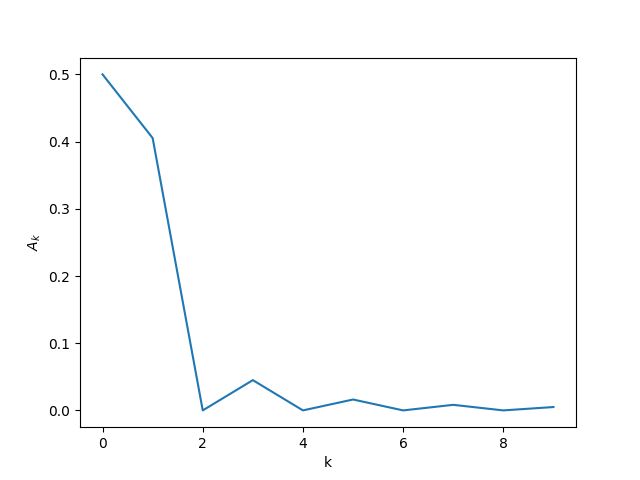
\includegraphics[width=8cm]{img/ex_5_b.png}
	\centering
\end{figure}

\textbf{c) Plot the Fourier series from [-T0;T0] for kmax = 1 and kmax = 9.}
\\

\lstinputlisting[language=Python, firstline=15]{code/ex_5.py}

\begin{figure}[H]
	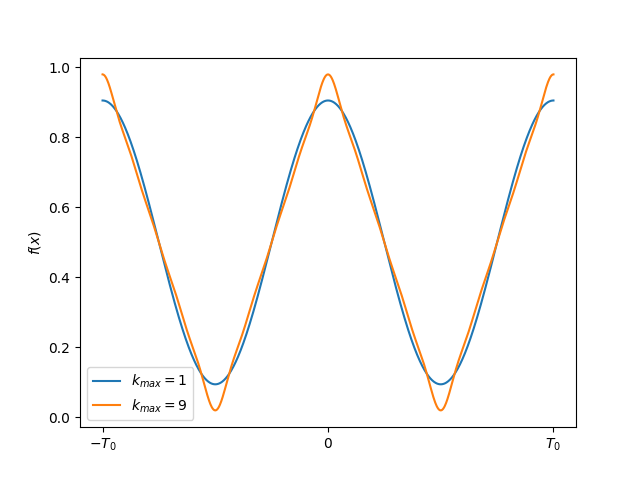
\includegraphics[width=8cm]{img/ex_5_c.png}
	\centering
\end{figure}
